\documentclass[crop,tikz]{standalone}
\usetikzlibrary{shapes}
\usetikzlibrary{arrows}
\usetikzlibrary{positioning}

\begin{document}
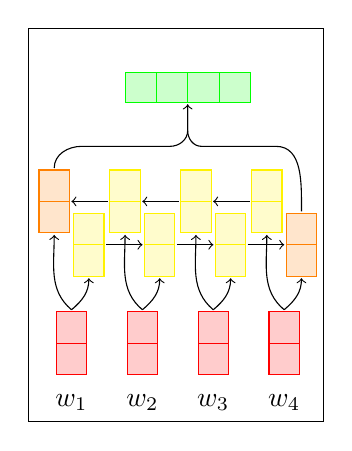
\begin{tikzpicture}[
  hid/.style 2 args={
    rectangle split,
    draw=#2,
    rectangle split parts=#1,
    fill=#2!20,
    outer sep=.25mm},
  mlp/.style 2 args={
    rectangle split,
    rectangle split horizontal,
    draw=#2,
    rectangle split parts=#1,
    fill=#2!20,
    outer sep=.25mm}
]

 % Comment out this line to remove border.
 \draw[draw=black] (0, 5) rectangle (3.75, 0);

 \foreach \step in {1,...,4} {
   \node (i\step) at (.9*\step -.35, .25) {$w_\step$};
   \node[hid={2}{red}] (e\step) at (.9*\step - .35, 1) {};    
 }

 \foreach \step in {1,...,4} {
   \node[hid={2}{yellow}] (hr\step) at (.9 *\step - .22 -.35, 2.8) {};    
   \node[hid={2}{yellow}] (hf\step) at (.9 *\step + .22 -.35, 2.25) {};    
 }
 \node[hid={2}{orange}] (hr1) at (.9 *1 - .22 -.35, 2.8) {};    
 \node[hid={2}{orange}] (hf4) at (.9 *4 + .22 -.35, 2.25) {};    
 \node[mlp={4}{green}] (s) at (.9 * 2.25, 4.25) {};

 \foreach \last/\next in {1/2, 2/3, 3/4} {
   \draw[->] (hf\last.east) -> (hf\next.west);
   \draw[->] (hr\next.west) -> (hr\last.east);
 }

 \foreach \step in {1,...,4} {
   \draw[->] (e\step.north) to [out=140,in=270] (hr\step.south); 
   \draw[->] (e\step.north) to [out=40,in=270] (hf\step.south); 
 }

 \draw[-] (hf4.north) to [out=90,in=0] (.9 * 3.25 + .22, 3.5) 
 to (2.2, 3.5) to [out=180,in=270] (.9 * 2.25, 3.7) to (s.south); 
 \draw[->] (hr1.north) to [out=90,in=180] (.9 - .22, 3.5) 
 to (1.8, 3.5) to [out=0,in=270] (.9 * 2.25, 3.7) to (s.south); 
 
\end{tikzpicture}
\end{document}
